\documentclass{article}

% Please use the following line and do not change the style file.
% \usepackage{icml2023_author_response}

% Recommended, but optional, packages for figures and better typesetting:
\usepackage{microtype}
\usepackage{graphicx}
% \usepackage{subfigure}
\usepackage{hyperref}       % hyperlinks
\usepackage{booktabs} % for professional tables
\usepackage{amsfonts}       % blackboard math symbols
\usepackage{nicefrac}       % compact symbols for 1/2, etc.

\usepackage{lipsum}
\usepackage{amsmath}
\usepackage{multirow}
\usepackage{subcaption}


\begin{document}
% Uncomment the following line if you prefer a single-column format
%\onecolumn
\paragraph{Response summary:}
We thank all the reviewers for their insightful comments. In this paper, we are concerned about the ``exact full conformal prediction" (exact full-CP). The exact full-CP for complex black box models is intractable and an efficient computational method does not exist. As of today, exact full-CP is possible for ordinary least square, LASSO and ridge regression. The exact full-CP of a SHIM is the first attempt to compute an exact full-CP set for a non-linear model. 
\vspace{0.5cm}

We believe that the ``exact full-CP" of a SHIM has significant importance in practice where accuracy, statistical reliability, and interpretability are important. We would appreciate it if the reviewers reconsider their decisions about our paper. 


\vspace{0.5cm}

\textbf{Paper presentation:} We will correct the typos and improve the presentation of the paper by taking into consideration of each and every comment and recommendation of all the reviewers.


 

\section*{Reviewer \#1}

\textbf{Q1. Why don't you show r-squared for HIV, friedman2, bodyfat?}\\

We did not include those results because of the space constraint. However, we could certainly include those results in the supplementary documents. We will definitely include the r-squared results for HIV, friedman2, bodyfat in the revised version. We want to make sure that the r-squared results for HIV, friedman2, bodyfat are consistent with what we observed in the conformal prediction (CP) set results. Indeed, if a model poorly fits to the data it leads to a poor r-squared value and a large CP set.\\

\begin{figure}[h!]
\begin{subfigure}{0.4\textwidth}
\centering
    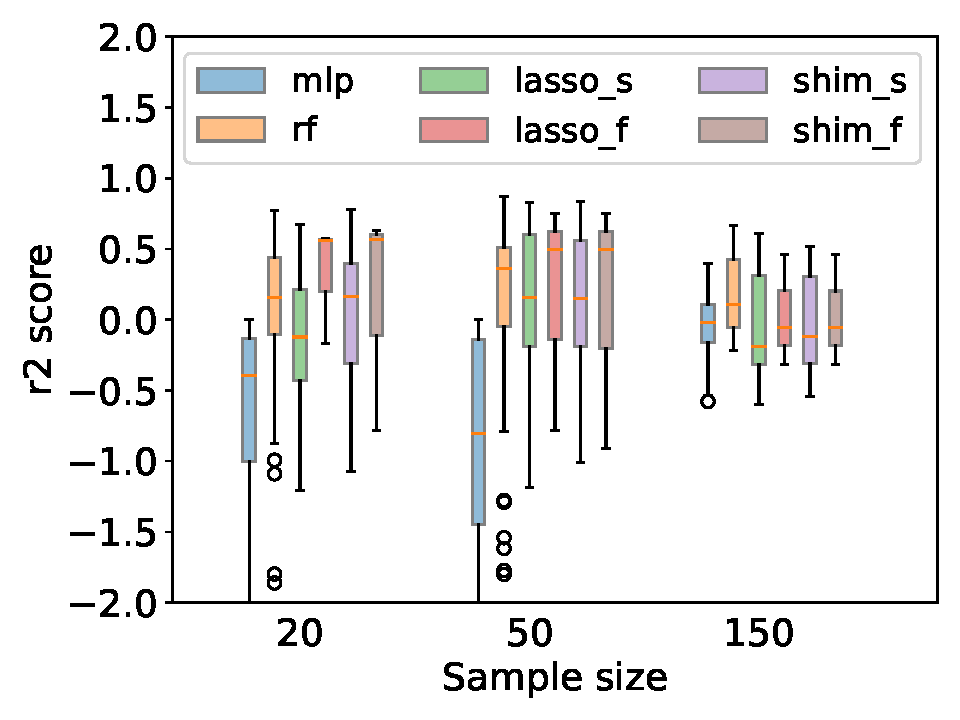
\includegraphics[width=\textwidth]{figures/r2_3tc_20_50_150_.pdf}
    \caption{3tc}
    \label{fig:1}
\end{subfigure}
\hfill
\begin{subfigure}{0.4\textwidth}
\centering
    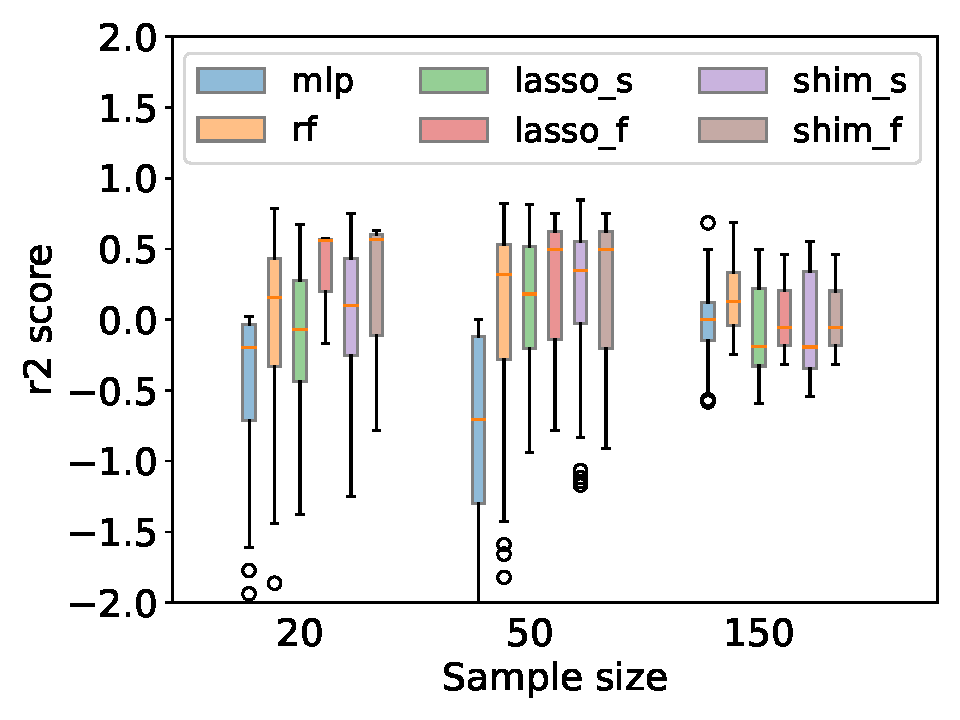
\includegraphics[width=\textwidth]{figures/r2_abc_20_50_150_.pdf}
     \caption{abc}
    \label{fig:2}
\end{subfigure}
\caption{Comparing of r2 scores of the proposed method (shim) with other simple (lasso) and complex (mlp, rf) models using HIV drug resistance data (3tc and abc).}
\end{figure}


\begin{figure}[h!]
\begin{subfigure}{0.4\textwidth}
\centering
    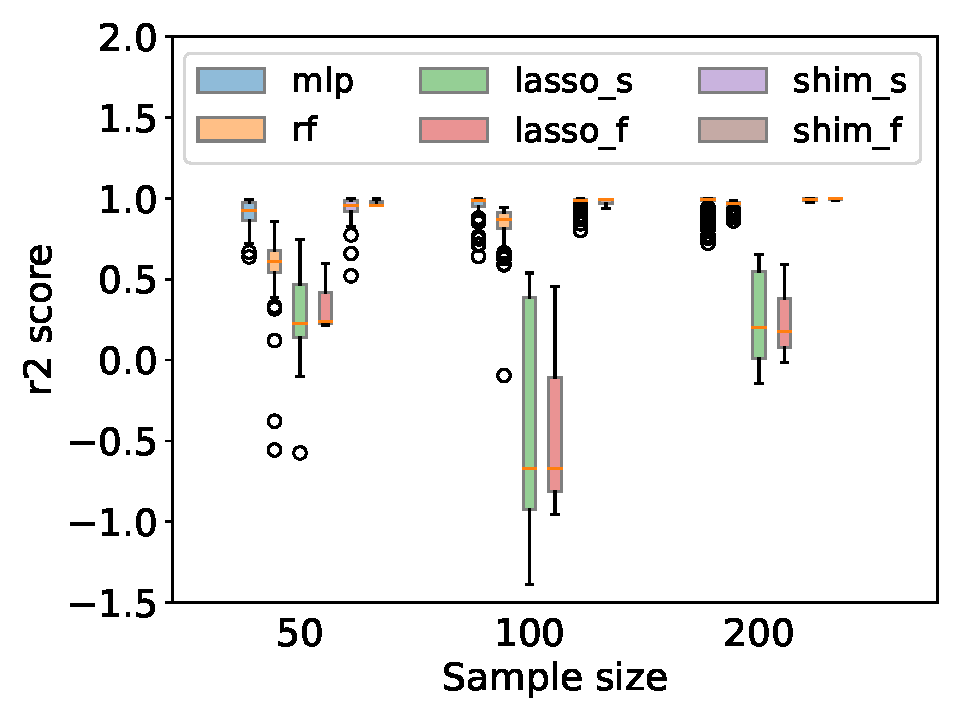
\includegraphics[width=\textwidth]{figures/r2_friedman2_continuous_50_100_200_.pdf}
    \caption{friedman2}
    \label{fig:1}
\end{subfigure}
\hfill
\begin{subfigure}{0.4\textwidth}
\centering
    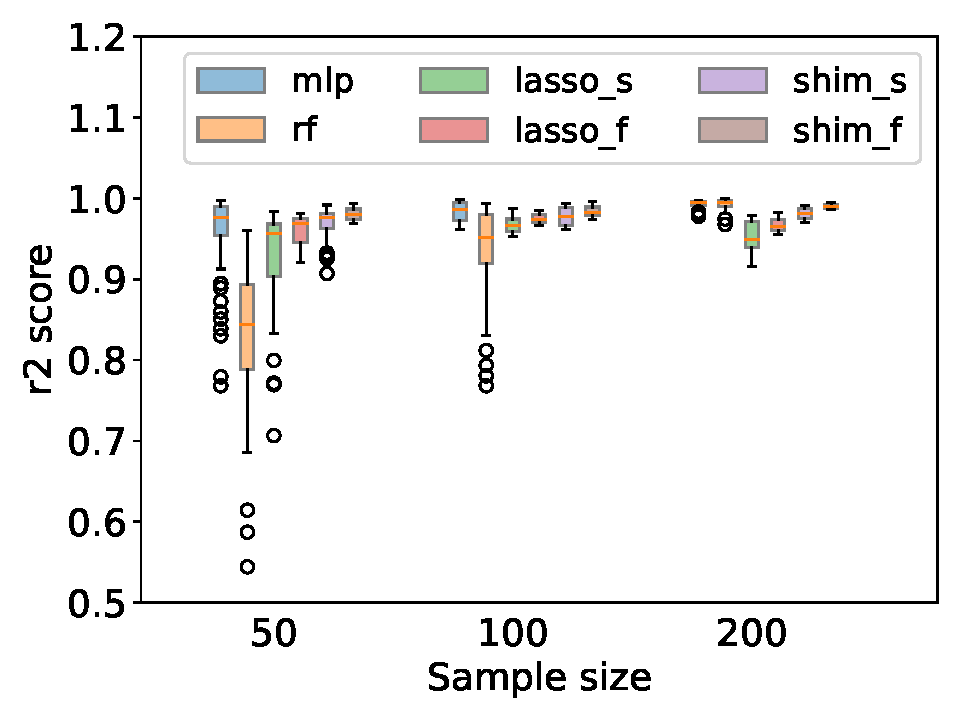
\includegraphics[width=\textwidth]{figures/r2_bodyfat_50_100_200__.pdf}
     \caption{bodyfat}
    \label{fig:2}
\end{subfigure}
\caption{Comparing of r2 scores of the proposed method (shim) with other simple (lasso) and complex (mlp, rf) models using continuous synthetic (friedman2) and real world (bodyfat) data.}
\end{figure}



%\begin{table}[h!]
%    \centering
%    \begin{tabular}{|c|c|c|c|c|c|c|c|}
%    \hline
%         &n &mlp &rf &lasso\_s &lasso\_f &shim\_s &shim\_f \\
%         \cline{2-8}
%          \multirow{2}{*}{$R^2$} &50 &0.90 ($\pm 0.08$)& 0.58 ($\pm 0.19$) &0.28 ($\pm 0.22$) &0.35 ($\pm 0.17$)  &0.93 ($\pm 0.07$)& 0.97 ($\pm 0.01$)\\
%         \cline{2-8}
%           &100 &0.95 ($\pm 0.07$)& 0.83 ($\pm 0.12$) &-0.41 ($\pm 0.63$) &-0.38 ($\pm 0.60$)  &0.97 ($\pm 0.03$)& 0.97 ($\pm 0.02$)\\
%         \cline{2-8}
%         &200 &0.96 ($\pm 0.05$)& 0.96 ($\pm 0.02$) &0.24 ($\pm 0.25$) &0.25 ($\pm 0.25$)  &0.99 ($\pm 0.01$)& 0.99 ($\pm 0.01$)\\
%         \hline
%    \end{tabular}
%    \caption{$R^2$ results for Table 4 (friedman2).}
%    \label{tab:rsquared_friedman2}
%\end{table}
%
%
%
%
%\begin{table}[h!]
%    \centering
%    \begin{tabular}{|c|c|c|c|c|c|c|c|}
%    \hline
%         &n &mlp &rf &lasso\_s &lasso\_f &shim\_s &shim\_f \\
%         \cline{2-8}
%          \multirow{2}{*}{$R^2$} &50 &0.95 ($\pm 0.04$)& 0.82 ($\pm 0.11$) &0.93 ($\pm 0.05$) &0.95 ($\pm 0.02$)  &0.97 ($\pm 0.01$)& 0.98 ($\pm 0.01$)\\
%         \cline{2-8}
%           &100 &0.98 ($\pm 0.01$)& 0.94 ($\pm 0.05$) &0.96 ($\pm 0.01$) &0.97 ($\pm 0.02$)  &0.97 ($\pm 0.01$)& 0.98 ($\pm 0.01$)\\
%         \cline{2-8}
%         &200 &0.99 ($\pm 0.01$)& 0.99 ($\pm 0.05$) &0.95 ($\pm 0.01$) &0.96 ($\pm 0.01$)  &0.98 ($\pm 0.01$)& 0.99 ($\pm 0.01$)\\
%         \hline
%    \end{tabular}
%    \caption{$R^2$ results for Table 4 (bodyfat).}
%    \label{tab:rsuared_bodyfat}
%\end{table}


\textbf{Q2. What are the sample size requirements for split-CP and why we don't want to use split-CP?}\\

Note that the naive approach of using the same full data both for fitting and calibration cannot be used as it violates the data exchangeability assumption of CP. Hence, a simple approach of split-CP has been devised where we can split the data into two parts: one part is used for model fitting and the other part is used for model calibration (i.e., CP set construction). The proportion of splitting depends on the user and the standard practise is to use 50:50 proportion. However, it is important to mention that there exists a trade off of model fitting vs model calibration depending on the splitting proportion. If we use more data in fitting then the model calibration will suffer due to small data size and similarly if we use more data in calibration then model will poorly fit to the data. Either way we will loose statistical efficiency (i.e., it will generate a larger CP set). The CP set generated by a split-CP also suffers from the randomness of data splitting as it can be seen in all the experimental results.\\ 


\textbf{Q3. SHIM performs well when the ground truth is itself a SHIM. How does it perform when the ground truth is not a SHIM?}\\

In Table 1 and Table 2, we can see that SHIM performs well when the true model is a SHIM. However, it also performs well in other non-linear model (Figure 4, Friedman2) when the true model is not necessarily a SHIM.\\



\section*{Reviewer \#2}
\textbf{Q1. Add a discussion of Algorithm2 to the main text of the paper for completeness.}\\

We accept the feedback of the reviewer and certainly add a discussion of Algorithm2 to the main text and improve the readability of the paper in the revised version.\\

\textbf{Q2. Experimental evaluation with high dimensional data:}\\

For a high dimensional setting we used $n=150$ and $m=100$. Note that in case of a high-order interaction model, even a $2^{nd}$ order or a $3^{rd}$ order interaction model will lead to $p=\sum_{d=1}^2 \binom{100}{d}=5050$ or  $p=\sum_{d=1}^3 \binom{100}{d}=166750$ respectively. Hence, this is clearly a $p\gg n$ experimental settings for a SHIM.\\



\textbf{Q3. Proposition 3.1 should be mentioned clearly in its statement that it is from Lei (2019):}\\

We have cited the corresponding reference Lei (2019) immediately before stating Proposition 3.1 (Line 196 - 198, col 2). However, we will make every effort to clearly state that the Proposition 3.1 is taken from Lei (2019) in the revised version.\\ 



\section*{Reviewer \#3}
\textbf{Q1. Tree definition for continuous data}\\

 The tree anti-monotonicity property which states that $x_{i\ell} \geq x_{i\ell^\prime}, \forall \ell^\prime \supset \ell, \forall i \in [n+1]$ is true for any feature $x_{i \ell} \in [0,1], \forall \ell \in [p]$, whether it is binary or continuous (as long as it is scaled between 0 and 1). We exploited this property to prove the pruning condition stated in Lemma 3.2 ( see A.1. Proof of Lemma 3.2 and Proposition A.2. in the Appendix). However, we will update the definition of the tree and include this tree anti-monotonicity property in the main text of the revised version of the paper.\\


\textbf{Q2. The maximum order of interaction is selected by the algorithm automatically.}\\

In our proposed method, the user can fix the order of interaction. This is useful (computationally efficient) in case of a very large dimensional problem and in domains where only up to certain order of interactions are sufficient to model the data. However, if no maximum order of interaction is specified, then our method will find the optimum order of interactions given the data. As the tree grows progressively, the irrelevant interactions are filtered out by the pruning condition and optimal interactions are found by the algorithm automatically.\\  

\textbf{Q3. Choice of $\lambda$.}\\

Given a single sample in practise, the choice of $\lambda$ should be done in a similar way as it is done in standard machine learning settings. One needs to make sure that the model fitting and model selection should not be done on the same data.\\


\textbf{Q4. What are the operating characteristics of SHIM in terms of interaction detection?}\\

Given a data, a SHIM is able to find all the interactions present in the data. In Table 1 and Table 2, we reported results for up to $3^{ord}$ interaction terms, as the lengths of CP sets and $r^2$ values did not improve much beyond that.


\section*{Reviewer \#4}
\textbf{Q1. Novelty of the paper.}\\

The proposed method is motivated by Das et al. but the problem we solved in our paper is completely different. In Das et al. the author considered homotopy-mining to construct the path in the direction of test statistics using the framework of conditional selective inference. However, in this paper we constructed the path of residual with a parameterized response in the context of conformal prediction. Additionally solving the problem for a SHIM is nontrivial due to the combinatorial complexity of high-order interaction terms. We solved the problem and provided a practical solution.\\

\textbf{Q2. Add A.2 and the pseudo code to the main text.}\\

We accept the feedback of the reviewer and certainly include A.2 and the pseudo code in the revised version.\\

\textbf{Q3\&4. How to apply the proposed method in the domain of $[0, 1]^n$? Is any binarization required?}\\

The proposed method is equally applicable to both binary as well as continuous data (as long as it is scaled between 0 and 1). We do not need binarization to apply our method to continuous data. Please also refer to our answer to Q1 of reviewer\#3. \\

\textbf{Q5. Choice of the order of interaction in the true model of synthetic data experiments.}\\

The choice of the order of interaction in the true model is mainly for the demonstration purpose. Our method is equally applicable to any chosen order of interaction.\\

\textbf{Q6. Compare performance on large dataset ($n>200$).}
\\

See the results in Table~\ref{tab:friedman2_large_n}.

\begin{table}[h!]
    \centering
    \begin{tabular}{|c|c|c|c|c|c|c|}
    \hline
         &mlp &rf &lasso\_s &lasso\_f &shim\_s &shim\_f \\
         \hline
         cov &0.12 ($\pm 0.06$)& 0.36 ($\pm 0.05$) &2.45 ($\pm 0.12$) &2.44 ($\pm 0.06$)  &0.24 ($\pm 0.04$)& 0.23 ($\pm 0.02$)\\
         \hline
          $R^2$ &0.998 ($\pm 0.01$)& 0.984 ($\pm 0.01$) &0.478 ($\pm 0.29$) &0.484 ($\pm 0.28$)  &0.994 ($\pm 0.01$)& 0.994 ($\pm 0.01$)\\
         \hline
    \end{tabular}
    \caption{Results using Friedman2 data for large sample size ($n=500$).}
    \label{tab:friedman2_large_n}
\end{table}

\textbf{C1. Definition of $\mathcal{S}_i(\tau)$}\\

The $\mathcal{S}_i, \forall i \in [n+1]$ is the absolute residual of the $i^{th}$ data point. To compute this residual we fit the model with all $n+1$ data points, hence the full design matrix is used. The absolute residual of each data point does not depend on the order of the data and hence $\pi(\tau)$ also does not depend on the order of the data. \\


\textbf{C2. Why split-CP is computationally more efficient?}
Note that to construct a full-CP set in a regression setting, one needs to fit the model infinite times for all possible values of $y \in \mathbb{R}$ on the regression line. The number of model fittings depends on $y$ and not on training sample size $n$. Hence, the naive computation of full-CP is prohibitive. Whereas, in case of a split-CP, one just needs to fit the model only once using the one part of the data and construct the CP set using the remaining part. That is why split-CP is computationally more efficient. \\   

\textbf{C3. The aggregate-CP provides an inflated confidence level of $1 - 2\alpha$. What is the problem?}\\

The choice of $\alpha \in [0,1]$ determines the level of confidence $(1-\alpha)$ we have in our prediction. This essentially determines the statistical efficiency (length of the CP set). A high confidence generally leads to a wider confidence set. For example, a $90\%$ confidence set is generally wider than a $80\%$ confidence set. Therefore, if we specify $\alpha=0.1$, then split-CP and full-CP guarantees a $(1-0.1)\times 100\%=90\%$ confidence set, whereas aggregate-CP can only guarantee a $(1-2\times 0.1)\times 100\%=80\%$ confidence set for the same $\alpha$. Therefore, if we want to ensure $90\%$ confidence in aggregate-CP, then this will lead to a wider confidence set. See results in Fig.~\ref{fig:jacknife1} and Fig.~\ref{fig:jacknife2}\\ 

\begin{figure}[h!]
\begin{subfigure}{0.4\textwidth}
\centering
    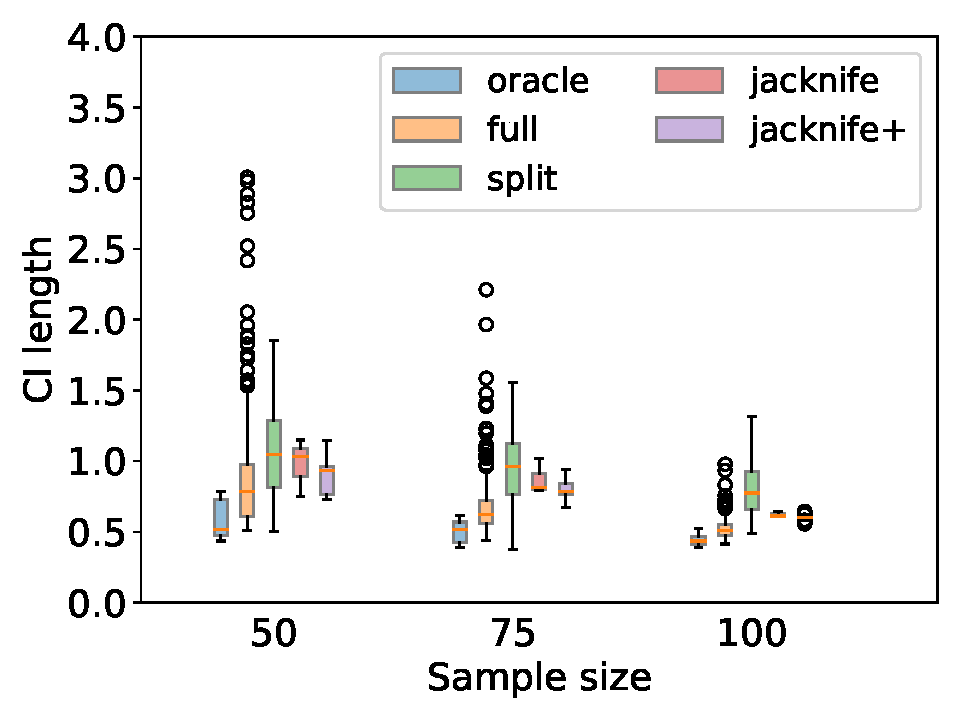
\includegraphics[width=\textwidth]{figures/cpl_ord_5_lmd_0.1_n_tr_50_75_100_.pdf}
    \caption{$\lambda=0.1$}
    \label{fig:jacknife1}
\end{subfigure}
\hfill
\begin{subfigure}{0.4\textwidth}
\centering
    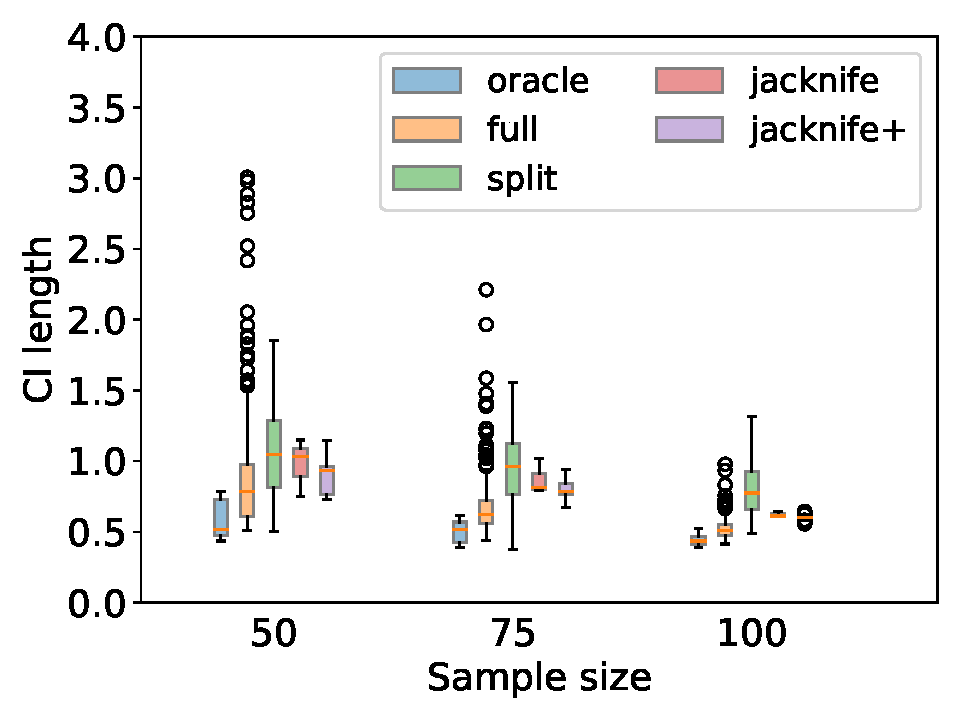
\includegraphics[width=\textwidth]{figures/cpl_ord_5_lmd_0.1_n_tr_50_75_100_.pdf}
     \caption{$\lambda=0.01$}
    \label{fig:jacknife2}
\end{subfigure}
\caption{Comparing confidence interval lengths (CI lengths) among different methods of CP set constructions (oracle, full, split, jacknife and jacknife+). Results using synthetic regression data for two different $\lambda$ values. We used \textbf{"sklearn.datasets.make\_regression"} to generate data. The following parameters have been used: n\_features=5, n\_informative=3, noise=1. $n_{train} \in [50, 75, 100]$ and $n_{test} = 100$. We repeated experiments $3$ times, hence we reported results of $3 \times 100 = 300$ test instances.}
\end{figure}

\textbf{C4. In Table 1 and 2, what do "s" and "f" mean in shim\_{2s} and shim\_{2f}?}\\

shim\_{2s} and shim\_{2f} respectively represent split-CP and full-CP for a $2^{nd}$ order SHIM. We will add this as a caption of Table 1 and 2 in the revised version of the paper as we did in the Figures 2, 3 and 4.\\



\end{document}
